\documentclass{pre-tfg}
\usepackage{longtable}

\title{Sistema de Guiado para Peatones, Ciclistas y Motoristas con Interacción Implícita}
\author{Carlos Ramos Mellado}
\advisorFirst{David Villa Alises}
\advisorDepartment{DEPARTAMENTO DE TECNOLOGÍAS Y SISTEMAS DE INFORMACIÓN}
\advisorSecond{}
\intensification{TECNOLOGÍAS DE LA INFORMACIÓN}
\docdate{2014}{Noviembre}


\begin{document}

\maketitle
\tableofcontents

\newpage

\section{INTRODUCCIÓN}

El guiado de personas es una actividad que se lleva desarrollando desde siempre con la
ayuda de las estrellas, mapas y brújulas. Afortunadamente para nosotros, en la actualidad
resulta sencillo seguir un determinado camino gracias a la navegación vía satélite. Aunque
existen varias tecnologías utilizadas para dicha navegación, hoy en día el \textit{Sistema
  de Posicionamiento Global}
(\textit{GPS}\footnote{https://es.wikipedia.org/wiki/Sistema\_de\_posicionamiento\_global})
de los Estados Unidos y el \textit{Sistema Orbital Mundial de Navegación por Satélite}
(\textit{GLONASS}\footnote{https://es.wikipedia.org/wiki/GLONASS}) de la Federación Rusa
son las únicas tecnologías operativas~\cite{SPSA}.

Con la popularización de los \emph{smartphones} se extendió el uso de la navegación vía
satélite y es común encontrar personas utilizándola por medio de aplicaciones como
\textit{Google
  Maps}\footnote{https://play.google.com/store/apps/details?id=com.google.android.apps.maps}
o
\textit{Sygic}\footnote{https://play.google.com/store/apps/details?id=com.sygic.aura}. Estas
aplicaciones resultan muy adecuadas para la navegación en trayectos en coche aunque
implican un requisito importante: es necesario ver la pantalla u oír las instrucciones
para llevarlas a cabo. Eso no es demasiado inconveniente en un coche, pero para los peatones,
ciclistas y motoristas el hecho de mirar a la pantalla o intentar oír el smartphone supone
una distracción que potencialmente puede provocar un accidente~\cite{Valcarcel12} y, por
tanto, necesitan otro tipo de interacción con el dispositivo.

Las distracciones del conductor son una de las principales causas de accidentabilidad en todo el mundo. La \textit{National Highway Traffic Safety Administration} (\textit{NHTSA}\footnote{http://www.nhtsa.gov/}) señaló en 2003 que la distracción de los conductores es la causa de 1,5 millones de accidentes producidos anualmente en todo el planeta \cite{RACC03}. Y, según un estudio de la aseguradora Allianz de 2014 \cite{Allianz14}, el 26\% de los accidentes por distracciones son producidos por mirar el navegador.

En España, el uso de dispositivos como navegadores, cascos y auriculares por parte del conductor está considerado como una infracción grave y acarrea una multa de 200 euros y una pérdida de 3 puntos en el carné de conducir \cite{Serrano14} .

En este trabajo se desarrollará un sistema de guiado en el que el usuario obtendrá realimentación del sistema sin necesidad de ver la pantalla. Para ello, el sistema avisará al usuario en el momento que tenga que realizar cualquiera de las acciones posibles: girar a izquierda, girar a la derecha, continuar recto o dar media vuelta. Esta interacción se llevará a cabo por medio de la vibración al igual que en los proyectos \cite{Boemo12} y \cite{Merino13}, o en las zapatillas \textit{Lechal} \cite{Lechal} . A parte del vibrador incorporado en el smartphone se utilizará un periférico como un smartwatch o pulsera inteligente. De este modo, cuando haya que girar a la izquierda vibrará uno, cuando haya que girar a la derecha vibrará el otro y cuando haya que dar media vuelta vibrarán ambos. En la Figura~\ref{fig:descipcion_sistema} se esquematiza un giro a la izquierda:

\begin{figure}[!h]
  \begin{center}
    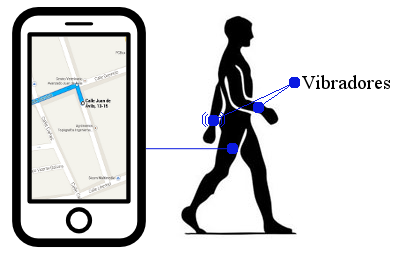
\includegraphics[width=0.6\textwidth]{girar-izquierda.png}
    \caption{Descripción del sistema. Giro a la izquierda}
    \label{fig:descipcion_sistema}
  \end{center}
  \vspace{-25pt}
\end{figure}

Para determinar con cuánto tiempo de antelación hay que avisar para que realice una acción se utilizará la velocidad a la que se desplace el usuario. De este modo nos aseguraremos de que tenga suficiente tiempo para reaccionar independientemente de la actividad que esté realizando: andar, ir en bici o moto.

Además se implementarán las opciones disponibles en todos los sistemas de guiado:

\begin{itemize}
  \item Visualización de la posición actual en el mapa mostrando en forma de circunferencia la precisión del geoposicionamiento proporcionado por los satélites.
  \item Superposición de la ruta seleccionada sobre el mapa. De este modo se podrá visionar la ruta a seguir antes de realizarse.
  \item Orientación automática del mapa dependiendo de la orientación del dispositivo. Haciendo uso del sensor de orientación del smartphone se rotará la imagen del mapa.
  \item Visualización por pantalla y reproducción sonora de las instrucciones a seguir. 
\end{itemize}

\newpage

\section{TECNOLOGÍA ESPECÍFICA / INTENSIFICACIÓN / ITINERARIO CURSADO POR EL ALUMNO}

En la Tabla~\ref{tab:tec-especifica} se muestra la tecnología especifica cursada por el alumno del Grado en Ingeniería Informática.

\begin{table}[hp]
  \centering
  \caption{Tecnología Específica cursada por el alumno}
  \label{tab:tec-especifica}

  \zebrarows{1}
  \begin{tabular}{l p{0.4\textwidth}}
    \multicolumn{2}{c}{\textbf{Marcar la tecnología cursada}} \\
    \hline
    X & Tecnologías de la Información \\
    ~ & Computación                   \\
    ~ & Ingeniería del Software       \\
    ~ & Ingeniería de Computadores    \\ \hline
  \end{tabular}
\end{table}

Del mismo modo, en la Tabla~\ref{tab:competencias} se enumeran las competencias más destacables de la intensificación cursada y la justificación de uso de esa competencia concreta dentro del proyecto.

\rowcolors{2}{tabrowbg}{}
\begin{spacing}{1.1}
\begin{longtable}{p{0.45\linewidth}p{0.45\linewidth}}
  \caption{Justificación de las competencias específicas abordadas en el TFG}
  \label{tab:competencias} \\

  \textbf{Competencia} & \textbf{Justificación} \\
  \hline
  \hline
    Capacidad para seleccionar, diseñar, desplegar, integrar, evaluar, construir, gestionar, explotar y mantener las tecnologías de hardware, software y redes, dentro de los parámetros de coste y calidad adecuados. & Se pretende crear un sistema de navegación, haciendo uso del hardware, software y las redes disponibles; con el mínimo coste y la mayor calidad posible.\\

    Capacidad para emplear metodologías centradas en el usuario y la organización para el desarrollo, evaluación y gestión de aplicaciones y sistemas basados en tecnologías de la información que aseguren la accesibilidad, ergonomía y usabilidad de los sistemas. & El diseño del sistema se centrará en el usuario para ratificar que se trata de un sistema accesible, usable y que adapta cómodamente al usuario.\\

    Capacidad de concebir sistemas, aplicaciones y servicios basados en tecnologías de red, incluyendo Internet, web, comercio electrónico, multimedia, servicios interactivos y computación móvil. & El sistema hará uso de servicios de navegación proporcionados en Internet, la procesará y dará al usuario la información necesaria para seguir su camino.\\

    Capacidad para comprender, aplicar y gestionar la garantía y seguridad de los sistemas informáticos. & El sistema deberá ser resistente a vulnerabilidades propias de la implementación ya que se seguirán las directrices expuestas en \cite{Moreno13}.\\

  \hline
\end{longtable}
\end{spacing}

\section{OBJETIVOS}

Puesto que la iteración con los navegadores vía satélite actuales se basan en el contacto
visual o mensajes auditivos, el trabajo consistirá en incorporar un nuevo tipo de
interacción implícita: la vibración. Por tanto, el objetivo que se pretende conseguir con
el trabajo es:

\begin{itemize}
\item Desarrollo de un sistema de navegación vía satélite que se
  comunique con el usuario por medio de la vibración de alguno de sus componentes
\end{itemize}

Este objetivo principal puede desglosarse en varios objetivos específicos:

\begin{itemize}
\item Estudio de las alternativas para interacción implícita
\item Desarrollo de la aplicación de navegación para smartphone
\item Búsqueda, selección e integración de de los complementos adecuados para
  interacción implícita
\end{itemize}

\section{MÉTODO Y FASES DE TRABAJO}

La metodología seleccionada para el desarrollo del trabajo ha sido una \textbf{metodología
  ágil}~\cite{Poole09}. Este tipo de metodología nos permite un mayor margen de maniobra
gracias a que los requisitos y las soluciones van evolucionando por medio del desarrollo
\textbf{iterativo e incremental}.

Para desarrollar el proyecto se ha dividido el trabajo en bloques cuyo resultado será
fundamental para realizar los siguientes. Por tanto, se pretende seguir un orden basado en
el siguiente:

\begin{description}
\item[Estudio del estado del arte] \hfill \\
  Se llevará a cabo un estudio preliminar que muestre los diferentes sistemas de
  navegación vía satélite actuales. Se mencionarán sus puntos fuertes y el método de
  interacción que tienen con el usuario. También se estudiará la posibilidad de incorporar
  otro medio de iteración en dichos sistemas de navegación.

\item[Desarrollo de la aplicación de navegación] \hfill \\
  En primer lugar, para el desarrollo de la aplicación, se realizará un estudio para
  seleccionar la \textbf{plataforma} sobre la que se desplegará. Puesto que intentamos que
  nuestro sistema llegue al mayor número de personas con el mínimo coste deberemos emplear
  la plataforma que más cuota de mercado tenga en dispositivos móviles. Probablemente
  \textbf{Android} \cite{Mercado}.

  En segundo lugar, tendremos que seleccionar alguna de las \textbf{tecnologías de
    geoposicionamiento}. Sería interesante usar
  \textit{Galileo}\footnote{https://es.wikipedia.org/wiki/Sistema\_de\_navegaci\%C3\%B3n\_Galileo}
  porque proporciona una mayor precisión pero, de momento, no es posible \cite{SPSA} . Por
  ello se usará la tecnología más extendida en nuestra región y en nuestros dispositivos
  móviles: \textbf{GPS}.

  También será necesario disponer de \textbf{mapas y rutas} para guiar al usuario. Para
  ello se estudiarán las dos alternativas más usadas \textbf{Google
    Maps}\footnote{https://www.google.es/maps/} y \textbf{Open Street
    Map}\footnote{http://www.openstreetmap.org/}; y se usará la que más se adapte a
  nuestras necesidades.

  Finalmente se procederá al desarrollo de la aplicación llevando a cabo un análisis de
  requisitos, un diseño y una implementación.

\item[Búsqueda, selección e integración de los dispositivos vibratorios] \hfill \\
  Existe una gran variedad de complementos vibratorios como pulseras, brazaletes,
  cuantificadores personales o, incluso,
  deportivas \cite{Lechal} . Debido
  a esta gran variedad de dispositivos, será necesario buscar los complementos del mercado
  que se puedan usar con la plataforma elegida en el bloque anterior y seleccionar el que
  más se adapte a nuestras necesidades. Si se diese el caso de que ningún complemento
  cumpla los requisitos, desarrollaremos nuestros propios vibradores.

  Finalmente se llevará a cabo la integración de los dispositivos vibratorios con la
  aplicación desarrollada en el bloque anterior.

\item[Pruebas] \hfill \\
  Se realizarán pruebas sobre los escenarios inicialmente planteados: peatones, ciclistas
  y motoristas; y se evaluará la eficacia del desarrollo.

\item[Documentación] \hfill \\
  Se escribirá la documentación relacionada con el proyecto en la que se incluirán todos
  los diagramas, diseños, manuales, etc; que se generen durante la realización del mismo.

\end{description}

\newpage

\section{MEDIOS QUE SE PRETENDEN UTILIZAR}

\subsection{Medios Hardware}

Para la realización del proyecto sólo se prevén necesarios tres dispositivos hardware:

\begin{itemize}
\item \textbf{Computador}: Para desarrollar la aplicación y generar la documentación
  emplearé mi ordenador portátil \textbf{Asus
    X54H}\footnote{http://www.asus.com/Notebooks\_Ultrabooks/X54H/}.
\item \textbf{Smartphone}: Para probar la aplicación durante el desarrollo y la etapa de
  pruebas utilizaré mi teléfono móvil \textbf{Nexus
    5}\footnote{https://www.google.es/nexus/5/}.
\item \textbf{Complementos vibratorios}: Para realizar la interacción implícita se usarán
  dos o más complementos vibratorios que aún están por determinar.
\end{itemize}

\subsection{Medios Software}

De igual modo, se prevén necesarios cuatro medios software:

\begin{itemize}
\item \textbf{Elementary OS Luna}\footnote{http://elementaryos.org/}: Sistema Operativo
  GNU/Linux del computador de desarrollo.
\item \textbf{Eclipse
    ADT}\footnote{https://developer.android.com/tools/sdk/eclipse-adt.html}: entorno de
  desarrollo seleccionado para llevar a cabo el proyecto porque incluye la API de Android.
\item \textbf{Git} \cite{Hinojosa14} : Sera utilizado como control de versiones por medio
  de un repositorio de Bitbucket\footnote{https://bitbucket.org/}.
  \item \textbf{\LaTeX} \cite{Lamport86} : Lenguaje de marcado de documentos que se
    utilizará para realizar la documentación con el programa
    LaTeXila\footnote{https://wiki.gnome.org/Apps/LaTeXila}.
\end{itemize}

\newpage

\section{REFERENCIAS}

\renewcommand\refname{}
\vspace{-1cm}

\bibliographystyle{ieeetr}
\bibliography{anteproyecto}

\end{document}


% Local Variables:
% coding: utf-8
% mode: flyspell
% ispell-local-dictionary: "castellano8"
% mode: latex
% End:
